\subsection{Boosted Event Selection}
In the boosted channel, the most important selection above the others is that at least one large R jet fulfils the W/Z boson $80\%$ efficiency working points. Then, those events are further categorized into high purity and low purity regions determined by whether the 50$\%$ working point is passsed. The full selection could be seen in Tab. \ref{tab:SRdefinitions}

\begin{table}[t]
	\caption{Summary of the selection criteria in the definition of the signal region (SR), $W$+jets control region ($W$ CR) and $t\bar{t}$ control region ($t\bar{t}$ CR), in the high-purity (HP) and low-purity (LP) categories.  } \label{tab:SRdefinitions}
	\begin{center}
		\begin{adjustbox}{center}
		\begin{tabular}{|l|l|c|c|c|c|c|c|}
			\hline
			\multicolumn{2}{|l|}{\multirow{2}{*}{Selection}} & \multicolumn{2}{c|}{SR}  &  \multicolumn{2}{c|}{$W$ CR}  & \multicolumn{2}{c|}{$t\bar{t}$ CR} \\
			\cline{3-8}
			\multicolumn{2}{|l|}{} & HP & LP &HP & LP & HP & LP \\
			\hline
			\multirow{4}{*}{$W\rightarrow l\nu$} & Num of signal leptons & \multicolumn{6}{c|}{ 1 } \\
			\cline{2-8}
			&Num of vetoed leptons & \multicolumn{6}{c|}{ 0 }  \\
			\cline{2-8}
			&\vphantom{\Large B} $E^{miss}_{T}$ & \multicolumn{6}{c|}{ $>100GeV$ } \\
			\cline{2-8}
			&$p_{T}(l\nu)$ & \multicolumn{6}{c|}{ $>200GeV$ } \\
			\hline
			\multirow{5}{*}{$W/Z\rightarrow J$} & Num of large-$R$ jets & \multicolumn{6}{c|}{ $\geq 1$ } \\
			\cline{2-8}
			& \vphantom{\Large B} $D^{(\beta=1)}_2$ 50\,\% WP & pass & fail & pass & fail & pass & fail \\
			\cline{2-8}
			& \vphantom{\Large B} $D^{(\beta=1)}_2$ 80\,\% WP & --- & pass  & --- & pass  & --- & pass \\
			\cline{2-8}
			& $W/Z$ mass 50\,\% WP & pass &fail& --- & --- & pass & fail\\
			\cline{2-8}
			& $W/Z$ mass 80\,\% WP &  --- & pass & fail & fail & --- & pass\\
			\hline
			\multirow{2}{*}{Topology cuts}
			& $p_{T}(l\nu) / m_{WV}$ & \multicolumn{6}{c|}{ \multirow{2}{*}{$>0.3 (0.4)$ for VBF (ggF) category } }\\
			& $p_{T}(J) / m_{WV}$  & \multicolumn{6}{c|}{} \\
			\hline
			Top-quark veto & Num of $b$-tagged jets & \multicolumn{4}{c|}{0} & \multicolumn{2}{c|} {$\geq 1$} \\
			\hline
			Multi-jet BG Cleaning Cut & $E_T^{miss} / p_T(lv) > 0.2$ & \multicolumn{6}{c|}{ Electron channel only } \\
			\hline
			\multicolumn{2}{|c|}{Existence of VBF jets} & \multicolumn{6}{c|}{ yes (no) for VBF (ggF) category } \\
			\hline
		\end{tabular}
	    \end{adjustbox}
	\end{center}
\end{table}
\noindent
\\For the leptonically decayed system, the requirement is that exactly one signal is selected with $E^{miss}_{T}$ above $100GeV$ to suppress the multijet background. The additional requirements on the system is two topological cuts on kinetic properties: 
\begin{itemize}
	\item (a) $E^{miss}_{T}/p_{T}(e,\nu)>0.2$
	\item (b) $p_{T}(e,\nu)>0.2/m{WV}>0.3(0.4)$ for VBF (ggF) category
\end{itemize}
(a) is only for the electron channel to reduced multijet background further in the concern of the jet-faked electrons, while (b) is to lower the SM background contribution for the energy balance between the leptonically and hadronically decayed systems. These criteria are consistent across signal and control regions. 
\\
\\In the side of the hadronically decayed boson is only the large R jet. In addition to the requirement in the last section, the high purity regions (HP) (for both signal and control regions) demand the fat jet boson-tagged at $50\%$ WP, and it is the most sensitive region to signal. For the events with fat jets failing $50\%$ but passing $80\%$ WPs, they went into the low purity region (LP), and the combined sensitivity of HP and LP signal regions could be improved by around $~10\%$. If the fat jet only fails mass cut and pass the $D_{2}^{\beta=1}$ of boson tagging, this event would not be discarded but be chosen into W+jet control region instead. Finally, $p_{T}$ of the fat jet is also required to be above $0.3(0.4)m_{WV}$ for the energy balance in VBF(ggF) category. The event categorization of signal and W+jet control regions for both high and low purity categories is illustrated in Fig. \ref{Fig:HPLPdefinitions}.
\begin{figure}[h]
	\centering
	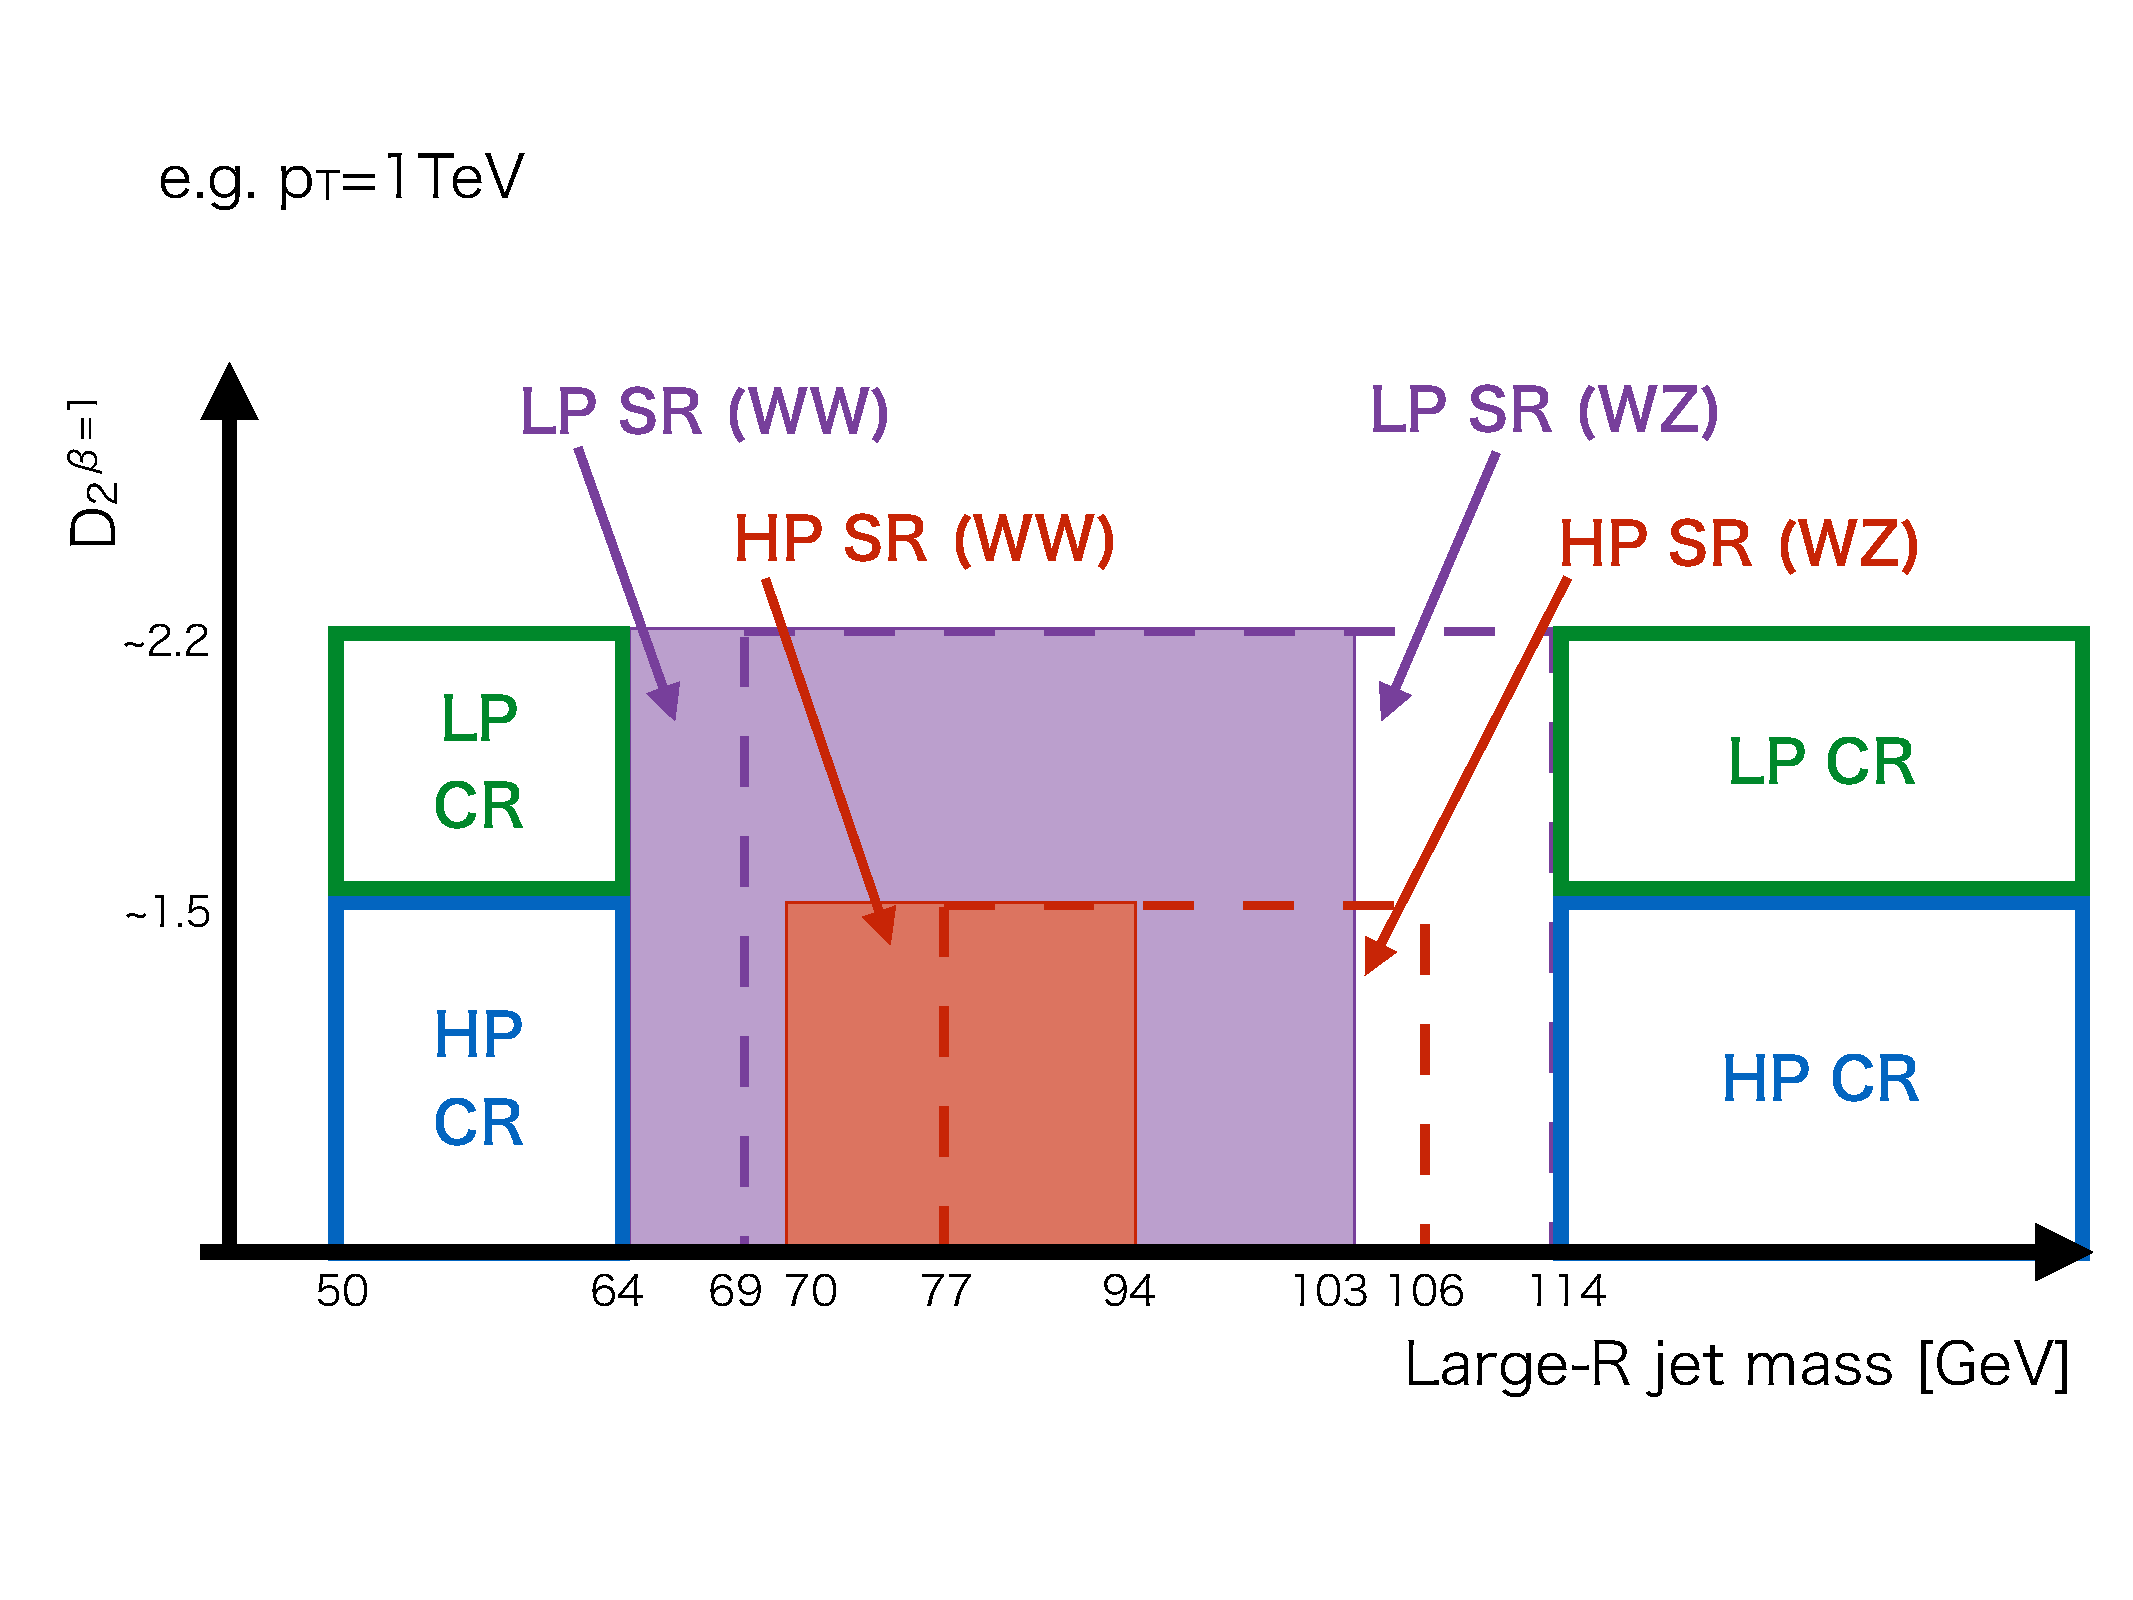
\includegraphics[width=0.8\hsize]{Chapter3/HPLPdefinitions}
	\caption{Definitions of signal region (SR) and $W$+jets control region (WR) for the event with the large-R jet of $\pt=1\,\TeV$ based on fat jet boson tagging and number of b-tagged jets }
	\label{Fig:HPLPdefinitions}
\end{figure}
\noindent
To reduce the $t\bar{t}$ background contribution, the subjets associated to the selected large R jet shall not be b-tagged in the W+jet control region and signal region. If any of them or the small R jets ($R=0.4$) pass the $85\%$ b-tagging WP, the event would go into the top control region. 
\\
\\Fig. \ref{Fig:HighPuritySR} and Fig. \ref{Fig:LowPuritySR} are the $m_{WV}$ distributions for the comparison of signal and background events in high purity and low purity signal regions for electron and muon channels respectively. 
\begin{figure}[h]
	\begin{center}
		\subfloat[]{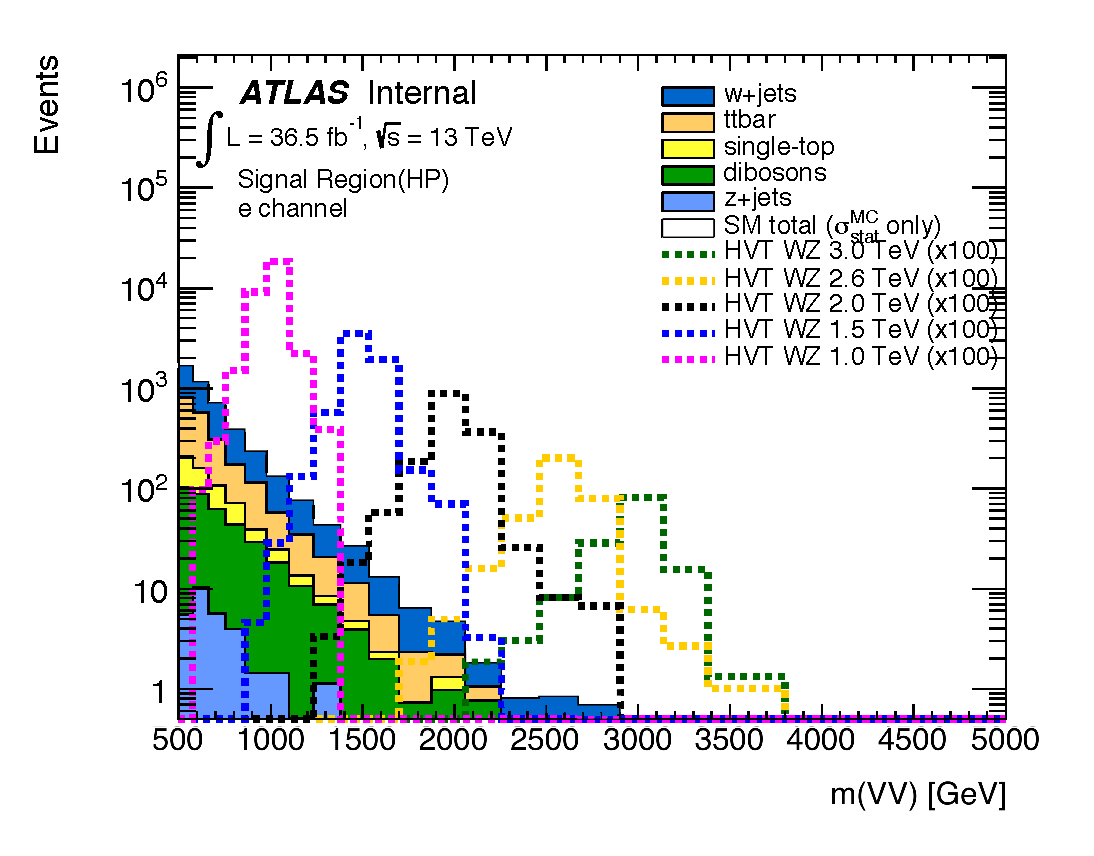
\includegraphics[width=0.5\hsize]{Chapter3/lvJmass_bveto_e.eps}}
		\subfloat[]{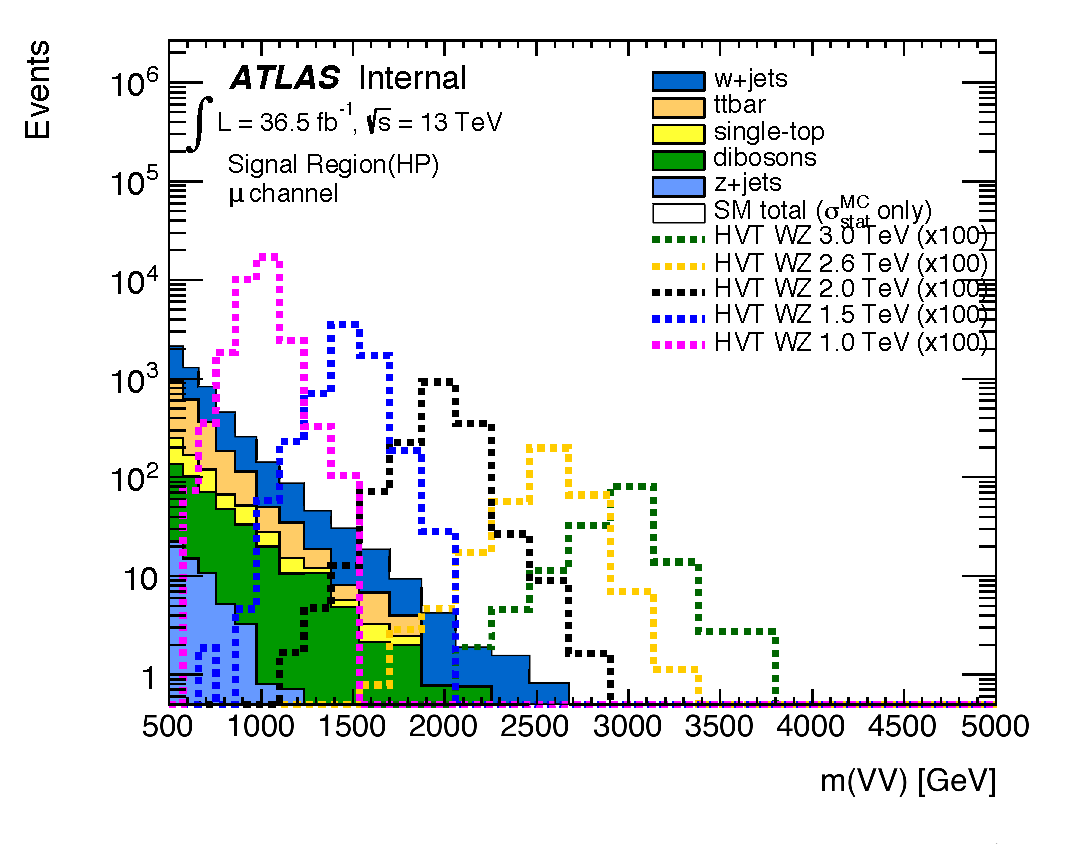
\includegraphics[width=0.5\hsize]{Chapter3/lvJmass_bveto_mu.eps}}
	\end{center}
	\caption{The $m_{WV}$ distributions in the HP signal region for (a) electron and (b) muon channel, with the integrated luminosity of $36.5fb^{-1}$. The HVT $WZ$ signals with $m=1.0TeV$, $1.5TeV$, $2.0TeV$, $2.6TeV$ and $3.0TeV$ are overlaid scaled to $100 ~\times$ cross section}
	\label{Fig:HighPuritySR}
\end{figure}

\begin{figure}[h]
	\centering
	\subfloat[]{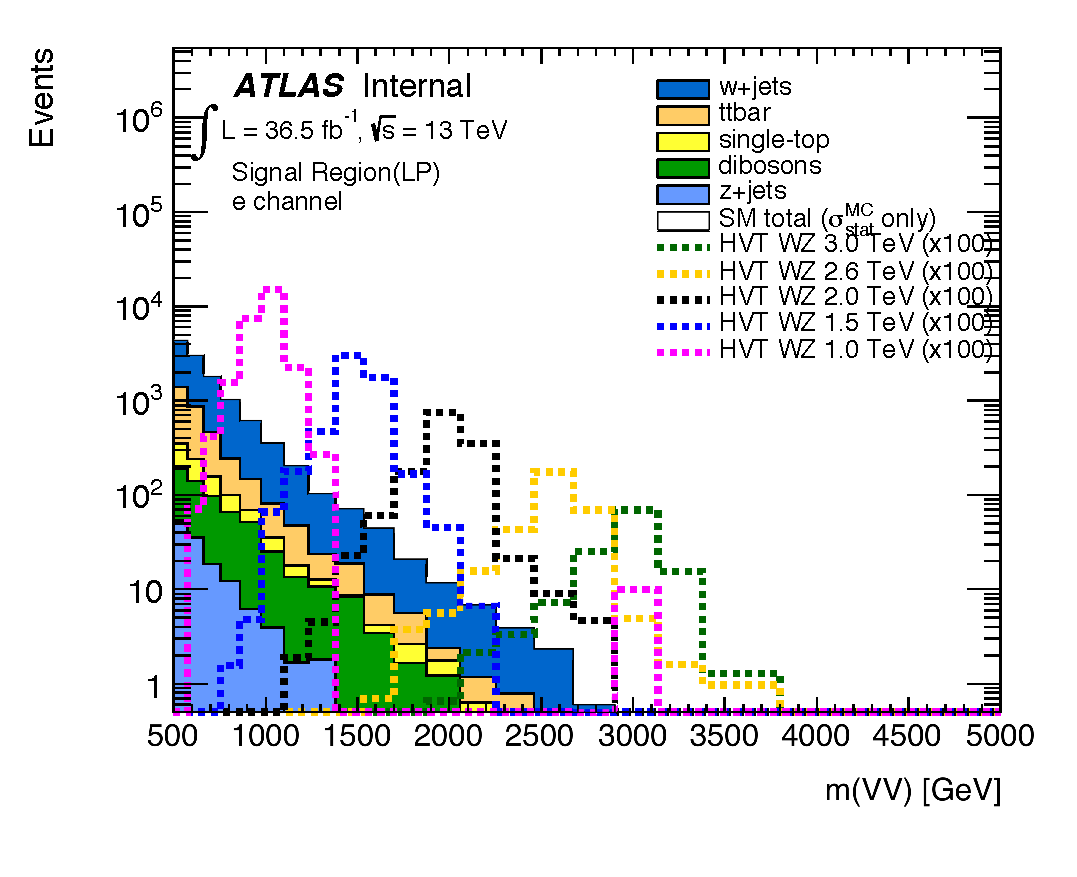
\includegraphics[width=0.5\hsize]{Chapter3/lvJmass_lowPurity_e.eps}}
	\subfloat[]{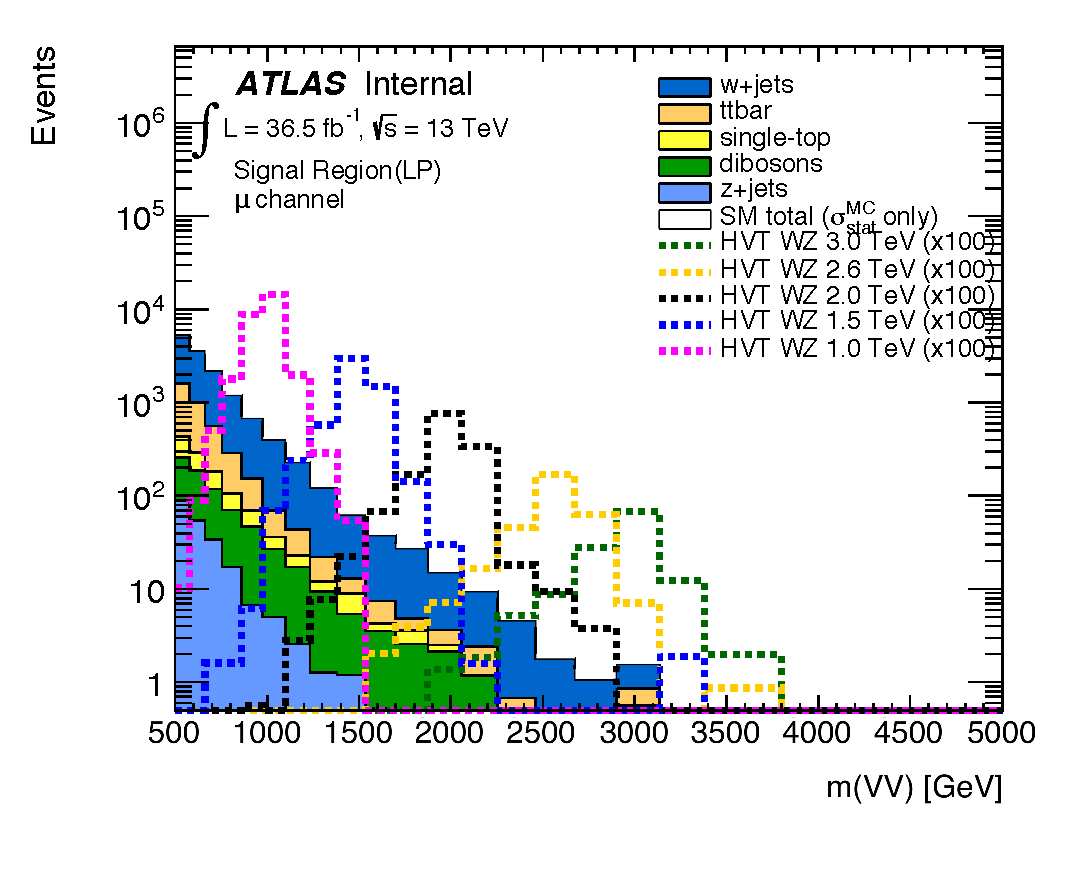
\includegraphics[width=0.5\hsize]{Chapter3/lvJmass_lowPurity_mu.eps}}
	\caption{The $m_{WV}$ distribution in the LP signal region for (a) electron and (b) muon channel, with the integrated luminosity of $36.5fb^{-1}$.The HVT $WZ$ signals with $m=1.0TeV$, $1.5TeV$, $2.0TeV$, $2.6TeV$ and $3.0TeV$ are overlaid 
	scaled to $100 ~\times$ cross section.}
	\label{Fig:LowPuritySR}
\end{figure}
%

\subsection{Resolved Event Selection}
Resolved channel has lower sensitivity than the boosted channel, but it still helps to recover the lost events in the lower energy regime. If the event has no fat jet fulfiling the selection criteria, it went to the resolved category. The full selection for both resolved signal and control regions could be seen in Tab. \ref{Tab:SRdefinitions_resolved}
\begin{table}[t]
	\caption{Summary of the selection criteria of of the  the resolved analysis for the $WW$ and $WZ$ signal regions (SR), $W$+jets control region (WR) and $ t\bar{t}$ control region (TR). } \label{Tab:SRdefinitions_resolved}
	\begin{center}
		\resizebox{\textwidth}{!}{
			\begin{tabular}{|l|l|c|c|c|c|}
				\hline
				\multicolumn{2}{|l|}{cuts} & $WW$ SR & $WZ$ SR & WR & TR \\
				\hline
				\multirow{3}{*}{$W\rightarrow \ell\nu$ selection} & Number of signal leptons & \multicolumn{4}{c|}{ 1 } \\
				\cline{2-6}
				&Number of veto leptons & \multicolumn{4}{c|}{ 0 }  \\
				\cline{2-6}
				&$E^{miss}_{T}$ & \multicolumn{4}{c|}{ $>60GeV$ } \\
				\cline{2-6}
				&$\pt(\ell\nu)$ & \multicolumn{4}{c|}{ $>75GeV$ } \\
				\hline
				\multirow{4}{*}{$W/Z\rightarrow jj$ selection} & Number of small jets & \multicolumn{4}{c|}{ $\geq2$ } \\ %$\geq 2$ & $\geq 2$ & $\geq 2$  \\
				\cline{2-6}
				& $\pt (j1)$ & \multicolumn{4}{c|}{ $>60$~GeV}\\
				\cline{2-6}
				& $\pt (j2)$ & \multicolumn{4}{c|}{ $>45$~GeV}\\
				\cline{2-6}
				& $m_{jj}$ & [66, 94]GeV\ & [82, 106]GeV\ & $<66GeV$ &  [66, 106]GeV \\
				&  &  &  & or [106, 200]GeV & \\
				\hline
				\multirow{6}{*}{Topology cuts} & $\Delta\phi(j,\ell)$ & \multicolumn{4}{c|}{ $>1.0$}\\
				\cline{2-6}
				& $\Delta\phi(j,E^{miss}_{T})$ & \multicolumn{4}{c|}{ $>1.0$}\\
				\cline{2-6}
				& $\Delta\phi(j,j)$ & \multicolumn{4}{c|}{ $<1.5$}\\
				\cline{2-6}
				& $\Delta\phi(l,E^{miss}_{T})$ & \multicolumn{4}{c|}{ $<1.5$}\\
				\cline{2-6}
				& $\pt(e\nu) / m_{WV}$ &\multicolumn{4}{c|}{\multirow{2}{*}{$>0.3 (0.35)$ for VBF (ggF) category}}\\
				& $\pt(jj) / m_{WV}$ & \multicolumn{4}{c|}{ } \\
				\hline
				\multirow{2}{*}{Top veto} & Number of $b$-tagged jets in $W/Z$ & $\leq 1$ & $\leq 2$ & $\leq 1$ & $\geq2$ \\
				\cline{2-6}
				& Number of other $b$-tagged jets & \multicolumn{3}{c|}{0} & or $\geq 1$ \\
				\hline
				\multicolumn{2}{|c|}{Existence of VBF jets} & \multicolumn{4}{c|}{ yes (no) for VBF (ggF) category } \\
				\hline
			\end{tabular}
		}
	\end{center}
\end{table}

Same to the boosted channel, the system of leptonically decayed W boson has a signal lepton fulfilling the object definition in last section. However, $E_{T}^{miss}$ cut here is lowered to $60GeV$ for the less energetic system as compared to the boosted channel. For the energy balance, the ratio between $p_{T}(l,\nu)$ and $m_{WV}$ shall be be over 0.3 (0.35) for VBF (ggF) category. 
\\
\\In the hadronic side, the two signal jets are selected after VBF jets, and they are required to have $p_{T}$ above $60GeV$ ($45GeV$) for the leading (subleading) one to suppress the SM background. As they are decayed from W or Z boson, their combined mass shall be within the dedicated mass windows, which are $[66, 94]GeV$ for the WW signal region and $[82, 106]GeV$ for the WZ signal region. Because the same top control region is used to make constraint in both of the two signal regions, the mass window is set at $[66,106]GeV$ as the OR condition of W and Z mass windows. For the events with the dijet mass falling into the side band region ($[0,66]GeV$ or $[106,200]GeV$), they are taken into the W+jet control. The energy balance requirement here is the same as the leptonic system: $p_{T}(jj)/m_{WV}>0.3(0.35)$ for VBF (ggF) category. 
\\
\\For the optimization of flavour tagging, the existence of b-jets increases the sensitivity in the resolved channel, so the jets could be b-tagged. In WW (WZ) signal region or W+jet control region, 1 (2) b-tagged jets can be found in the signal jets, but the presence of more b-tagged jets in addition to the signal jets would make the event go to the top control region.
\\
\\Different from the boosted channel, it has abundant background contribution from multijet background (details in next section), so a series of topological cuts are applied on the signature topology to further suppress it, which are listed below:
\begin{itemize}
	\item $\Delta\phi(j,l)>1.0$
	\item $\Delta\phi(j,E^{miss}_{T})>1.0$
	\item $\Delta\phi(j,j)<1.5$
	\item $\Delta\phi(l,E^{T}_{miss})<1.5$
\end{itemize}
The optimization was studied with dijet ($jj\rightarrow jj$) MC sample. 
\\
\\Fig. \ref{Fig:ResolvedSR} is the $m_{WV}$ distributions for comparison of signal and background in resolved signal regions for ggF and VBF categories respectively. The signal samples are with lower mass, because resolved channel has better sensitivity to them. 
\begin{figure}[h]
	\centering
	\subfloat[]{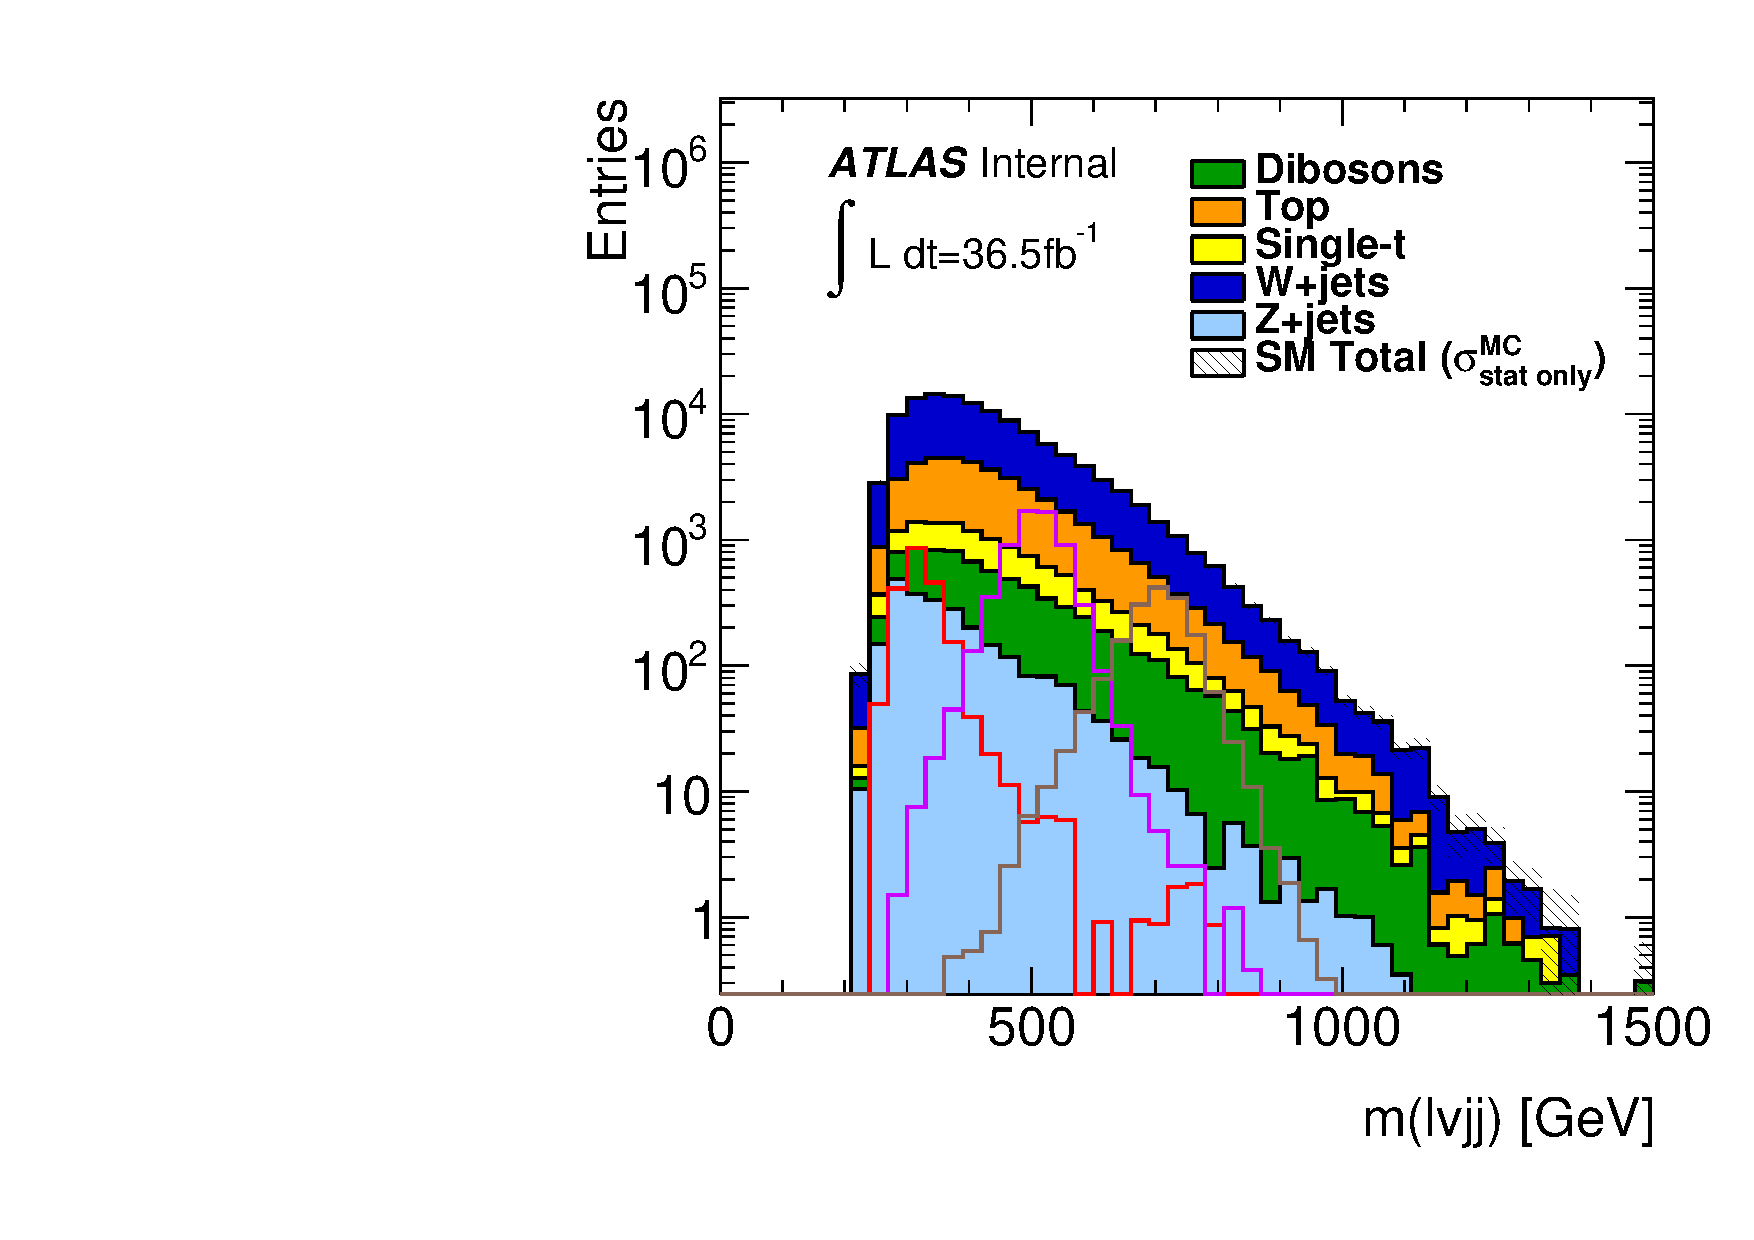
\includegraphics[width=0.5\hsize]{Chapter3/lvjjmass_ggF}}
	\subfloat[]{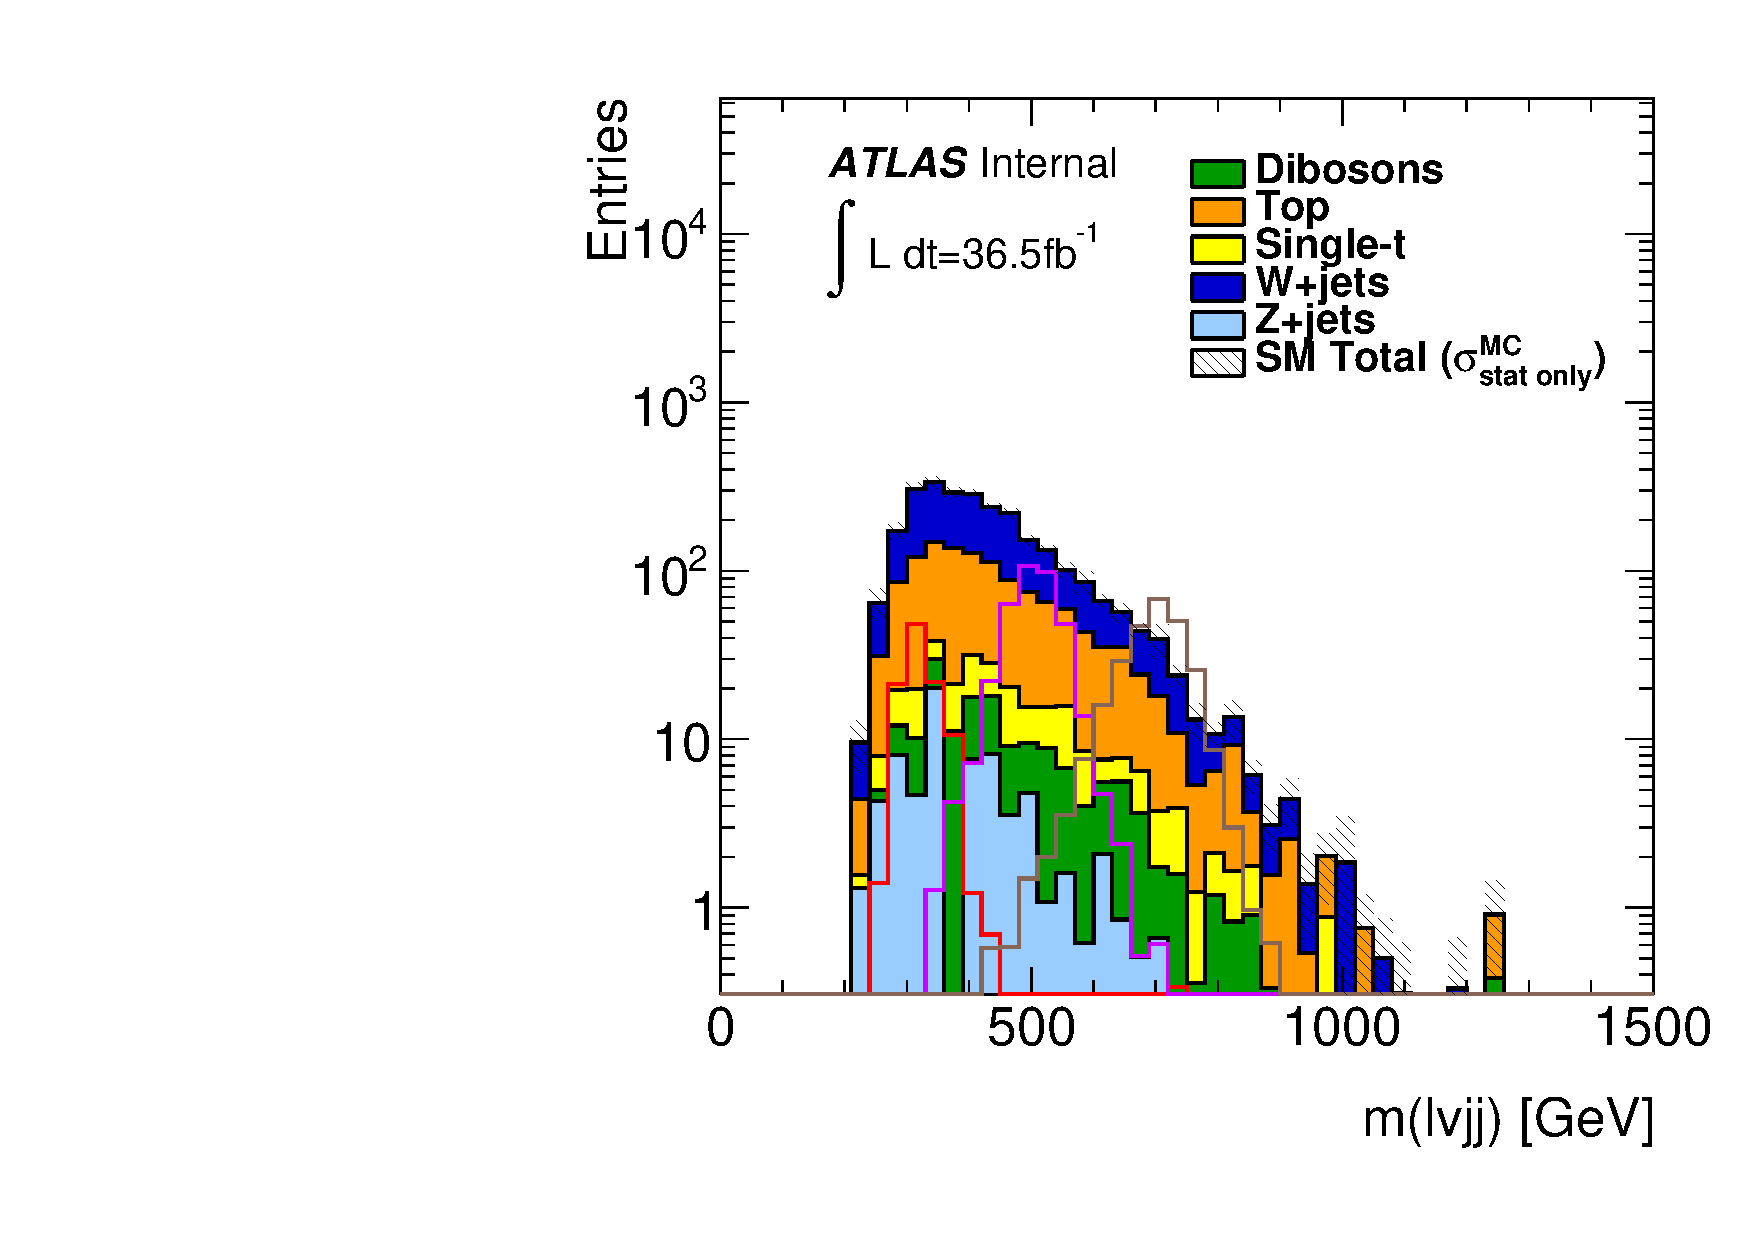
\includegraphics[width=0.5\hsize]{Chapter3/lvjjmass_VBF}}
	\caption{The $m_{WV}$ distribution in the resolved signal region for (a) ggF and (b) VBF channel, with the integrated luminosity of $36.5fb^{-1}$.The HVT $WZ$ signals with $m=300GeV$ (red), $500GeV$ (violet) and $700GeV$ (blue) are overlaid 
		scaled to $100 ~\times$ cross section.}
	\label{Fig:ResolvedSR}
\end{figure}
